\documentclass[border=1pt, tikz, convert={outext=.png}]{standalone}
\usepackage[rm]{roboto}
%\usepackage[rm,light]{roboto}

\usetikzlibrary{positioning, fit, decorations.text}
%\tikzset{every picture/.style={/utils/exec={\sffamily}}}
\tikzset{every picture/.style={line width=1pt}}

\definecolor{kts-blue}{RGB}{237,241,251}

\begin{document}
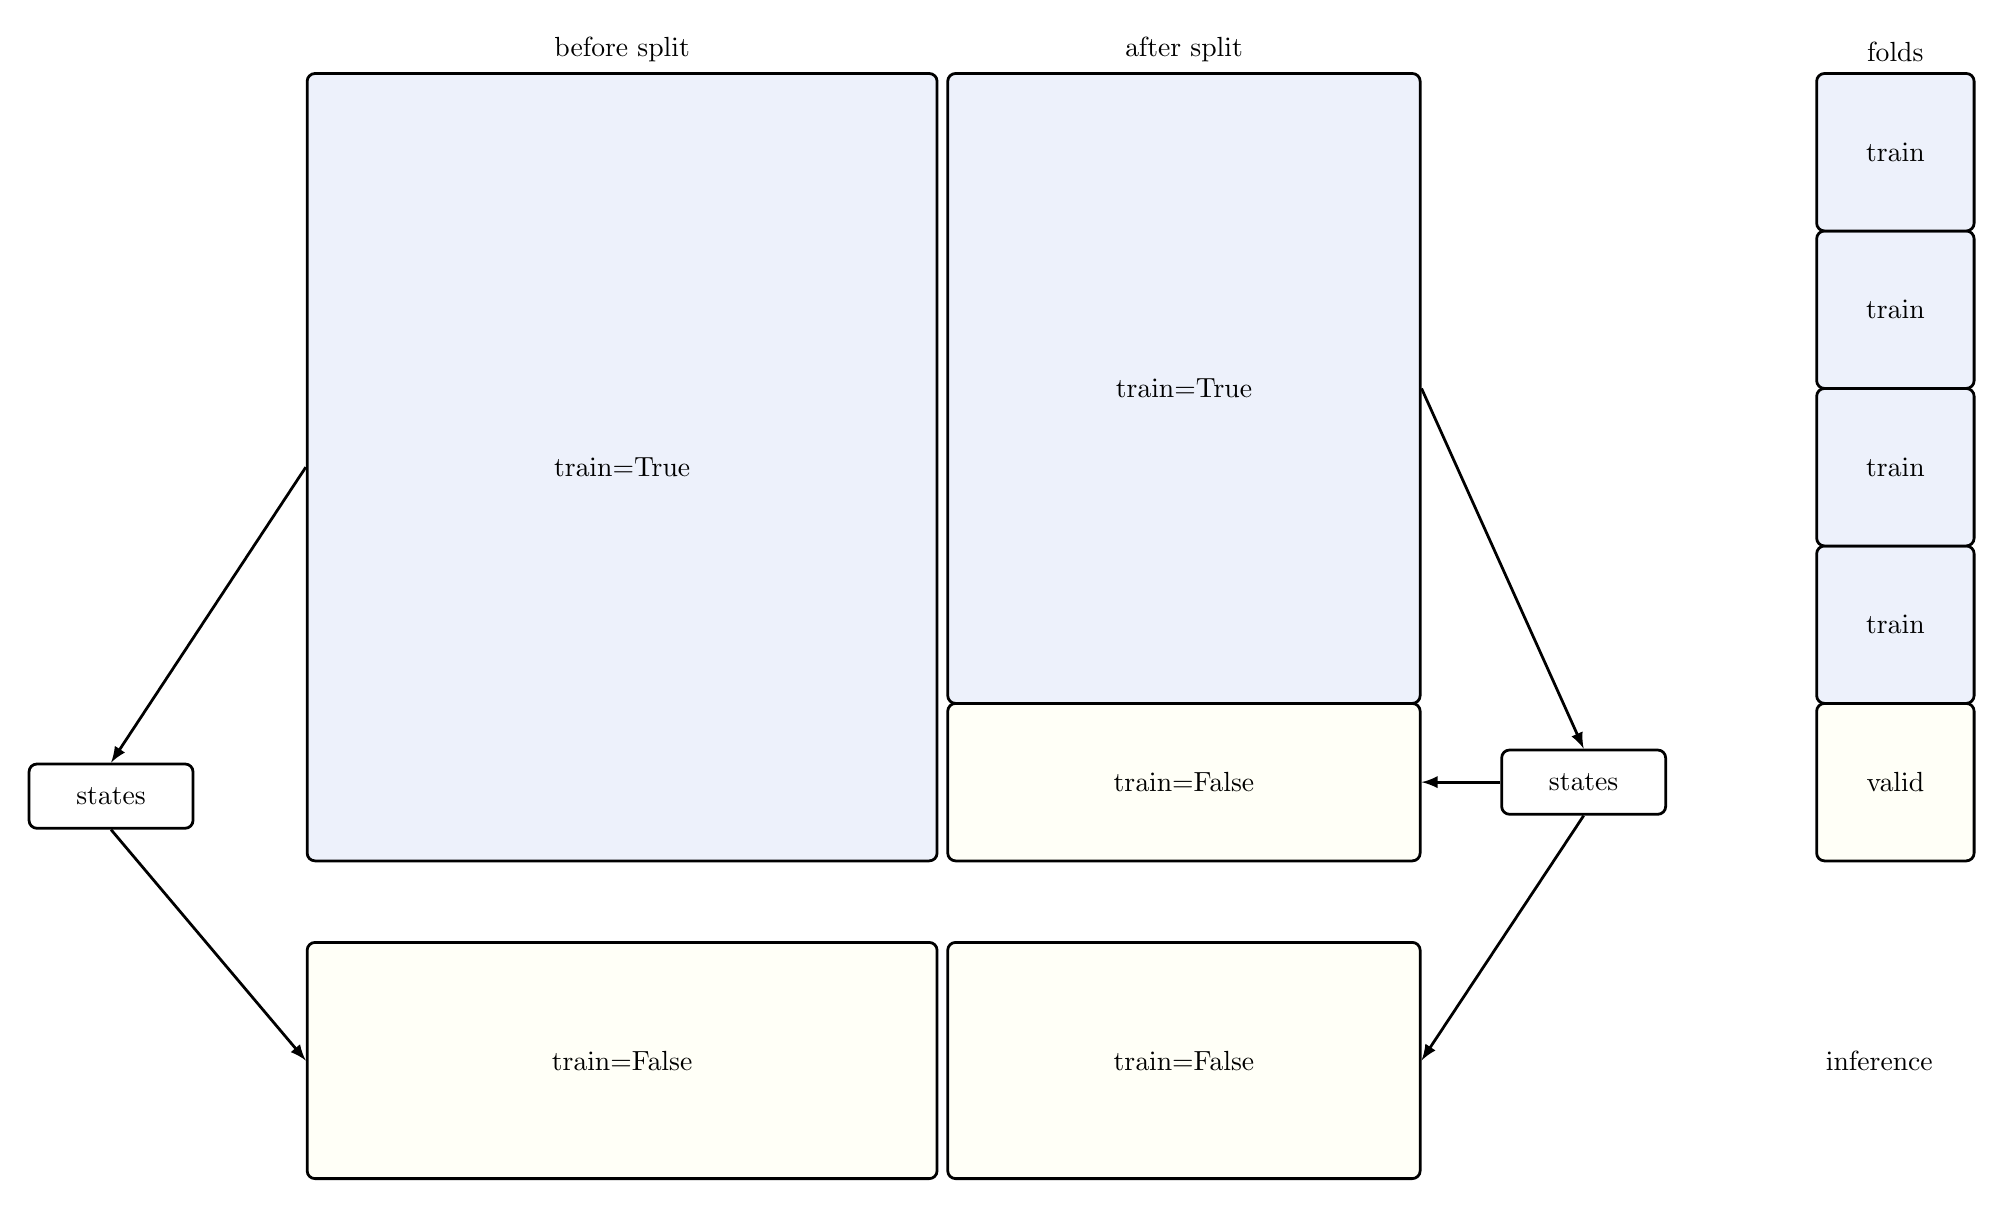
\begin{tikzpicture}
    [rect/.style = {rectangle, draw, align=center, 
            inner xsep=6mm, inner ysep=3mm, fill=kts-blue, rounded corners=0.1cm},
    -latex,     
    fs/.style = {rectangle, draw, align=center, 
            rounded corners=0.1cm},
    -latex,  
    ]
    
    
	\node[rect, minimum height=10cm, minimum width=8cm] (bef-train) at (0, 0) {train=True};
	
	\node[rect, minimum height=3cm, minimum width=8cm, below=1cm of bef-train, fill=yellow!3] (bef-inf) {train=False};
	
	
	\node[rect, minimum height=3cm, minimum width=6cm, right=0.1cm of bef-inf, fill=yellow!3] (aft-inf) {train=False};
	
	\node[rect, minimum height=2cm, minimum width=6cm, above=1cm of aft-inf, fill=yellow!3] (aft-test) {train=False};
	
	\node[rect, minimum height=8cm, minimum width=6cm, above=-1pt of aft-test] (aft-train) {train=True};
	
	
	\node[rect, minimum height=2cm, minimum width=2cm, right=5cm of aft-test, fill=yellow!3] (fold0) {valid};
	\node[rect, minimum height=2cm, minimum width=2cm, above=-1pt of fold0] (fold1) {train};
	\node[rect, minimum height=2cm, minimum width=2cm, above=-1pt of fold1] (fold2) {train};
	\node[rect, minimum height=2cm, minimum width=2cm, above=-1pt of fold2] (fold3) {train};
	\node[rect, minimum height=2cm, minimum width=2cm, above=-1pt of fold3] (fold4) {train};
	
	\node[right=5cm of aft-inf] {inference};
	
	
	\node[above=0.0cm of bef-train] {before split};
	\node[above=0.0cm of aft-train] {after split};
	\node[above=0.0cm of fold4] {folds};
	
	
	\node[rect, above left=2cm of bef-inf, fill=none] (bef-states) {states};
	\node[rect, right=1cm of aft-test, fill=none] (aft-states) {states};
	
	\draw (bef-train.west) to (bef-states.north);
	\draw (bef-states.south) to (bef-inf.west);
	
	\draw (aft-train.east) to (aft-states.north);
	\draw (aft-states.west) to (aft-test.east);
	\draw (aft-states.south) to (aft-inf.east);
\end{tikzpicture}
\end{document}